\documentclass[10pt,a4paper]{article}
\usepackage[utf8]{inputenc}
\usepackage[spanish]{babel}
\usepackage{amsmath}
\usepackage{amsfonts}
\usepackage{amssymb}
\usepackage{makeidx}
\usepackage{graphicx}
\usepackage{lmodern}
\usepackage{kpfonts}
\usepackage[left=2cm,right=2cm,top=2cm,bottom=2cm]{geometry}
\begin{document}
\begin{center}

\includegraphics[scale=0.2]{imagenes/upzmg.png} 
\end{center}
\large \huge Fabian canales ochoa, ING. Mecatroica 7-A \\ \\
\large \huge \textbf{Operador Jacobiano.
} \\ \\
\begin{huge}
En cálculo vectorial, se llama jacobiano o determinante jacobiano al determinante de la matriz jacobiana. Tanto la matriz jacobiana como el determinante jacobiano reciben su nombre en honor al matemático Carl Gustav Jacobi.

En geometría algebraica, el jacobiano de una curva hace referencia a la variedad jacobiana, un grupo y variedad algebraica asociada a la curva, donde la curva puede ser embebida.
\end{huge}
\begin{huge}
La matriz jacobiana es una matriz formada por las derivadas parciales de primer orden de una función. Una de las aplicaciones más interesantes de esta matriz es la posibilidad de aproximar linealmente a la función en un punto. En este sentido, el jacobiano representa la derivada de una función multivariable.

Propiamente deberíamos hablar más que de matriz jacobiana, de diferencial jacobiana o aplicación lineal jacobiana ya que la forma de la matriz dependerá de la base o coordenadas elegidas. Es decir, dadas dos bases diferentes la aplicación lineal jacobiana tendrá componentes diferentes aún tratándose del mismo objeto matemático. La propiedad básica de la "matriz" jacobiana es la siguiente, dada una aplicación cualquiera.
\end{huge}
\\ \\
\begin{huge}
Función escalar
Empecemos con el caso más sencillo de una función escalar  . En este caso la matriz jacobiana será una matriz formada por un vector fila que coincide con el gradiente. Si la función admite derivadas parciales para cada variable puede verse que basta definir la "matriz" jacobiana como: la imagen 1.2
\end{huge}
 \begin{center}
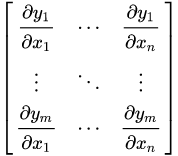
\includegraphics[scale=1.2]{imagenes/escalar.png} imagen 1.2
\end{center}
 mas ejemplos sobre matriz jacobiana se ven reflejados en la imagen 1.3 y 1.4:
 \begin{center}
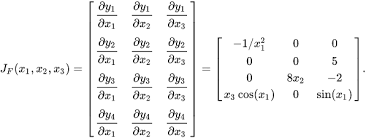
\includegraphics[scale=1.3]{imagenes/descarga.png} imagen 1.3
\end{center}
\begin{center}
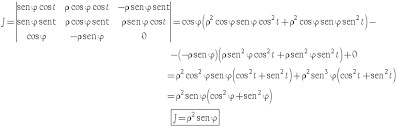
\includegraphics[scale=1.3]{imagenes/jacobiano.png} imagen 1.4
\end{center}
 \begin{huge}
 Una propiedad interesante del jacobiano es que cuando éste es diferente de cero en el entorno de un punto dado, entonces el teorema de la función inversa garantiza que la función admite una función inversa alrededor de dicho punto. un  ejemplo se muestra a continuacion
 \end{huge}
\begin{center}
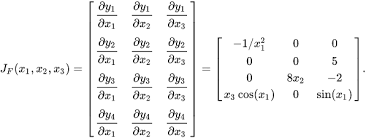
\includegraphics[scale=1.4]{imagenes/intervalo.png} imagen 1.4
\end{center}
\begin{Huge}
 \textbf{Referencias}
\end{Huge}
\\\begin{large}
 @phdthesis{ribeiro2010modelagem,
  title={Modelagem cinem{\'a}tica de sistemas rob{\'o}ticos cooperativos: proposta de uma jacobiano de coopera{\c{c}}ao},
  author={RIBEIRO, LUIZ PAULO GOMES},
  year={2010},
  school={Tese (Doutorado)—Universidade Federal de Santa Catarina, Florian{\'o}polis, Brasil}
}
\end{large}
\end{document}